%*****************************************
\chapter{Field Research}\label{ch11:field_research}
%*****************************************
%TODO Status: Pre-draft

\section{Introduction}

\begin{wrapfigure}{r}{0.4\textwidth}
	\centering
	
\includegraphics[width=0.4\textwidth]{gfx/11-mop} 
\end{wrapfigure}

If researchers wanted to know who conducts more of the housework in households, how could they find the answer? One way might be to interview people and simply ask them. That is exactly what Arlie Hochschild did in her study of the second shift, her term for the work that goes on in the home after the day's work for pay is completed\cite{hochschild2012second}. Hochschild interviewed $ 50 $ heterosexual, married couples with children to learn about how they did, or did not, share the work of the second shift. Many of these couples reported to her that they shared the load of the second shift equally, sometimes dividing the house into areas that were ``her responsibility'' and those that were ``his.'' But Hochschild was not satisfied with just people's personal accounts of second-shift work. She chose to observe $ 12 $ of these couples in their homes as well, to see for herself just how the second shift was shared.\blfootnote{Photo by rawpixel on Unsplash}

What Hochschild discovered was that even those couples who claimed to share the second shift did not have as equitable a division of duties as they had professed. For example, one couple who told Hochschild during their interview that they shared the household work equally had explained that the wife was responsible for the upstairs portion of the house and the husband took responsibility for the downstairs portion. Upon conducting observations in this couple's home, however, Hochschild discovered that the upstairs portion of the house contained all the bedrooms and bathrooms, the kitchen, the dining room, and the living room, while the downstairs included a storage space and the garage. This division of labor meant that the woman actually carried the weight of responsibility for the second shift. Without a field research component to her study, Hochschild might never have uncovered these and other truths about couples' behaviors and sharing (or not sharing) of household duties.

\begin{center}
	\begin{objbox}{Objectives}
		\begin{itemize}
			\setlength{\itemsep}{0pt}
			\setlength{\parskip}{0pt}
			\setlength{\parsep}{0pt}
			
			\item Define ``Field Research.''
			\item Describe the strengths and weaknesses of field research.
			\item Describe how to get started with field research: choosing a site and role.
			\item Describe how to write field notes and then analyze those notes.
		\end{itemize}
	\end{objbox}
\end{center}


\section{What Is Field Research?}

Field research is a qualitative method of data collection aimed at understanding, observing, and interacting with people in their natural settings. Thus when researchers talk about being in ``the field,'' they’re talking about being out in the real world and involved in the everyday lives of the people they are studying. Sometimes researchers use the terms ethnography or participant observation to refer to this method of data collection; the former is most commonly used in anthropology, while the latter is used commonly in sociology. This text uses two main terms: field research and participant observation. Field research is an umbrella term that includes the myriad activities that field researchers engage in when they collect data: they participate, they observe, they usually interview some of the people they observe, and they typically analyze documents or artifacts created by the people they observe.

Because interviews (Chapter \ref{ch10:interviews}) and document analysis (Chapter \ref{ch12:unobtrusive}) are covered elsewhere, this chapter focuses only on the participation and observation aspects of field research. These aspects of field research are usually referenced together and are known as participant observation. Like field research, participant observation also has multiple meanings. Researchers conducting participant observation vary in the extent to which they participate or observe \cite{baker2006observation}. While many ``participation scales'' have been developed, Baker proposes a continuum where ``Nonparticipation'' lies at one end and ``complete membership'' lies at the other, as illustrated in Figure \ref{11:fig01}.

\begin{center}
	\begin{figure}[H]
		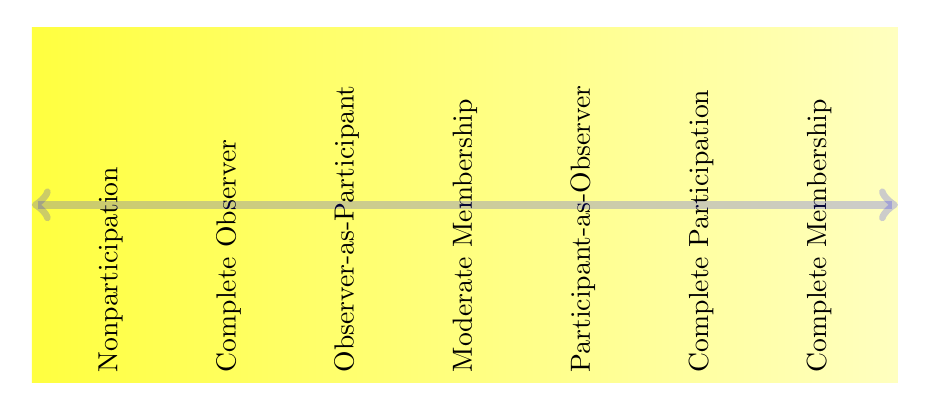
\begin{tikzpicture}
		% Yellow Rectangle
		\shade[left color=white!25!yellow, right color=white!75!yellow] (0,0) rectangle +(11cm, 4.5cm);

		% Text Nodes
		\tikzset{anchor=west}
		\node[rotate=90] at (1cm,0) {Nonparticipation};
		\node[rotate=90] at (2.5cm,0) {Complete Observer};
		\node[rotate=90] at (4.0cm,0) {Observer-as-Participant};
		\node[rotate=90] at (5.5cm,0) {Moderate Membership};
		\node[rotate=90] at (7.0cm,0) {Participant-as-Observer};
		\node[rotate=90] at (8.5cm,0) {Complete Participation};
		\node[rotate=90] at (10cm,0) {Complete Membership};

		% Horizontal Arrow
		\draw [<->, blue, line width=3pt, opacity=0.2] (0cm,2.25cm) to (11cm,2.25cm);
		
		\end{tikzpicture}
		\caption{Participant Observation Levels}
		\label{11:fig01}
	\end{figure}
\end{center}


\begin{description}

	\item[Nonparticipation] Researchers using this method have no involvement with the group being studied. Researchers are not physically present but can observe using an entirely different environment. As an example of this level of involvement, imagine a researcher watching some sort of group interaction from another room on a closed-circuit television system.

	\item[Complete Observer] Researchers using this method are physically present with the insiders being observed but have no interaction (or, at most, minimal superficial interaction) with the insiders. Researchers are only present to listen and observe.

	\item[Observer-as-Participant] Researchers using this method are engaged in more observation than participation but still have some interaction, like brief interviews, with the insiders. Researchers do not become friends with the insiders and would not ``get a beer after work'' but would feel comfortable asking them why they were doing some task in a particular manner. 

	\item[Moderate Membership] Researchers using this method attempt to maintain a balance between being an insider and pure observation. They would participate in certain activities but not those that are at the core of insider membership. As an example, researchers observing drug dealers may ``hang out'' and listen to music with them, but would not engage in any sort of illegal activity.

	\item[Participant-as-Observer] Researchers using this method become more involved with insiders' central activities but still do not fully commit to the members' values and goals. Researchers may develop friendships with the insiders and even participate in social activities, like going to dinner together, with them.

	\item[Complete Participation] Researchers using this method are said to ``go native'' with the insiders. They become part of the insiders' group and share all of the goals and norms of the group being studied. This level of involvement can be problematic since researchers may become so ingrained in the group being observed that they can no longer offer unbiased observations. For this reason, most research experts warn that ``going native'' should be avoided.

	\item[Complete Membership] Researchers using this method have completely ``gone native'' and are part of the group being observed. The main difference between this level and the previous level is that researchers who attain complete membership do so intentionally and have no hesitation in being part of the group being observed.

\end{description}

As it might have been imagined based on the examples of the observational roles assumed, field research is well equipped to answer ``how'' kinds of questions. Whereas survey researchers often aim to answer ``why'' questions, field researchers ask how the processes they study occur, how the people they spend time with in the field interact, and how events unfold. 

Field research is a method that was originally crafted by anthropologists for the purpose of cultural understanding and interpretation \cite{wolcott1999ethnography}. Dissatisfied with studying groups of people based solely on secondhand accounts and inspection of artifacts, several anthropologists decided to try living in or near the communities they studied to learn from and about them. Two anthropologists in particular, Franz Boas \cite{boas1964central} and Bronislaw Malinowski \cite{malinowski2014argonauts} are credited with developing this method around the turn of the 20th century. Boas lived with native populations in Canada and in the American Northwest. Malinowski lived in Papua New Guinea with people who were native to the area. Sociologists picked up on the idea and on the benefits of field research. Soon, a number of sociologists had embraced this new method and adapted field research for their own studies of groups. Many of the early field researchers in sociology were former social workers who got interested in sociological research because of experiences in their roles as social reformers. 

\section{Strengths and Weaknesses of Field Research}

Field research has many benefits, as well as a set of drawbacks, both explored here.

\subsection{Strengths of Field Research}

Field research allows researchers to gain firsthand experience and knowledge about the people, events, and processes that they study. No other method offers quite the same kind of closeup lens on everyday life. This close-up on everyday life means that field researchers can obtain very detailed data about people and processes, perhaps more detailed than they can obtain using any other method.

Field research is an excellent method for understanding the role of social context in shaping people's lives and experiences. It enables a greater understanding of the intricacies and complexities of daily life. Field research may also uncover elements of people's experiences or of group interactions of which we were not previously aware. This in particular is a unique strength of field research. With other methods, such as interviews and surveys, respondents cannot answer questions to which they do not know the answer or to provide us with information of which they are not aware. Also, because field research typically occurs over an extended period of time, social facts that may not even be immediately revealed to a researcher but that become discovered over time can be uncovered during the course of a field research project.

In sum, the major benefits of field research are the following:

\begin{enumerate}
	\item It yields very detailed data.
	\item It emphasizes the role and relevance of social context.
	\item It can uncover social facts that may not be immediately obvious or of which research participants may be unaware.
\end{enumerate}

\subsection{Weaknesses of Field Research}

Despite the fact that field researchers can collect very detailed data, that comes at a cost. Because a field researcher's focus is so detailed, it is by necessity also somewhat narrow. Field researchers simply are not able to gather data from as many individuals as, say, a survey researcher can reach. Indeed, field researchers generally sacrifice breadth in exchange for depth. Related to this point is the fact that field research is extremely time intensive.

Field research can also be emotionally taxing. Interview research requires, to a certain extent, the development of a relationship between a researcher and her participants, but field research requires a much greater investment in the researcher's life. It may be said that interviews are like casual dating while field research is like a marriage.

The relationships developed as a field researcher are sustained over a much longer period than the hour or two it might take to conduct an interview. Not only do the relationships last longer, but they are also more intimate. A number of field researchers have documented the complexities of relationships with research participants (See Taylor\cite{taylor2011intimate}, Sanjari\cite{sanjari2014ethical}, and Greene\cite{greene2014inside}). On the plus side, these relationships can be very rewarding (and yield the rich, detailed data noted as a strength in the preceding discussion). But, as in any relationship, field researchers experience not just the highs but also the lows of daily life and interactions. And participating in day-to-day life with one's research subjects can result in some tricky ethical quandaries. It can be a challenge if the goal is to observe as ``objectively'' as possible.

Finally, documentation can be challenging for field researchers. Where survey researchers have the questionnaires participants complete and interviewers have recordings, field researchers generally have only themselves to rely on for documenting what they observe. This challenge becomes immediately apparent upon entering the field. It may not be possible to take field notes as they observe, nor will they necessarily know which details to document or which will become the most important details to have noted. Finally, the notes taken after some observation may be incomplete since researchers may not recall everything exactly.

In sum, the weaknesses of field research include the following:

\begin{enumerate}
	\item It may lack breadth; gathering very detailed information means being unable to gather data from a very large number of people or groups.
	\item It may be emotionally taxing.
	\item Documenting observations may be more challenging than with other methods.
\end{enumerate}

\section{Getting In}

When embarking on a field research project, there are two major things researchers must consider: where to observe and what role to take at the field site. The decision about each of these will be shaped by a number of factors, some of which researchers will have control over and others which they will not. The decisions about where to observe and what role to play will also have consequences for the data they are able to gather and how that data are analyzed and shared.

\subsection{Choosing a Site}

Where to observe may be determined somewhat by the research question, but because field research often works inductively, researchers may not have a totally focused question before they begin observations. In some cases, field researchers do not define a research question until after they find out where the data are taking them. Other times, they begin with a research question but remain open to the possibility that their focus may shift as they gather data. In either case, when a site is chosen, a number of factors must be considered. What do they hope to accomplish with the field research? What is their topical/substantive interest? Where are they likely to observe behavior that has something to do with that topic? How likely is it that they will actually have access to the locations that are of interest? How much time do they have to conduct participant observations? Will the participant observations be limited to a single location or will they observe multiple locations?

Perhaps the best place to start as researchers identify a site or sites for their field research is to think about their limitations. One limitation that could shape participant observation is time. Field researchers typically immerse themselves in their research sites for many months, sometimes even years (see, for example, Davies\cite{davies2010corporate} and Jack\cite{jack2010entrepreneurial}). Researchers must ask themselves if they have several years available to conduct research or should they seek a smaller-scale field research experience? How much time do they have to participate and observe per day? Per week? Identifying the time available helps them determine where and what sort of research sites to choose.

Researchers must also think about where they live and whether travel is an option. Some field researchers actually move to live with or near their population of interest, but that may not be an option in most cases. Professor Erik Larson’s research on variations in economic institutions in a global environment, for example, has taken him across the globe, from Fiji to Ghana to Iceland\cite{larson2010time}. Sociologist Sara Dorow's research on transnational adoption took her from the United States to China\cite{dorow2006racialized}. These are just two of many examples of researchers who have traveled the globe for the purpose of collecting data. 

In choosing a site, researchers must also consider how the social location might limit what or where they can study. The ``ascribed'' aspects of locations are those that are involuntary, such as the researcher's age, race, or mobility. How might the ascribed status of a middle-aged man, for example, shape a researcher's ability to conduct complete participation in a study of children's birthday parties? The ``achieved'' aspects of locations, on the other hand, are those over which researchers have some control. In field research, researchers may also have some choice about whether or the extent to which they reveal the achieved aspects of their identities. There are numerous examples of field researchers whose achieved statuses granted them access to field sites into which they might not have otherwise been allowed. For example, a licensed paralegal may be able to gain access to law offices that would not be possible for other people.

The preceding discussion should not be taken to mean that researchers cannot, should not, or do not study those from whom they differ. In fact there have been plenty of successful field studies conducted by researchers who may have looked out of place in the sites they chose to investigate. Teresa Gowan, a self-described ``small, white English woman'' conducted field research with homeless men in some of San Francisco's most notoriously rough neighborhoods\cite{gowan2010hobos}. The aim here is not to reify the socially constructed categories upon which society places so much emphasis in organizing itself. Rather, the point is to be aware of which ascribed and achieved aspects of the researcher's identity may shape decisions about field sites.

Finally, in choosing a research site, researchers must consider whether the research will be a collaborative project or completed on their own. Collaborating with others has many benefits; researchers can cover more ground and therefore collect more data than if they are working on their own. Also, having collaborators in any research project, but especially field research, means having others with whom researchers can share their trials and tribulations in the field. However, collaborative research comes with its own set of challenges such as possible personality conflicts among researchers, competing commitments in terms of time and contributions to the project, and differences in methodological or theoretical perspectives. When considering something that is of interest, researchers should consider whether they have possible collaborators and how those collaborators could shape the decisions about where to conduct participant observation.

While this section began by considering the limitations that might shape field site decisions, it is also true to remember the opportunities\textemdash social, geographic, and otherwise\textemdash that location affords. Perhaps researchers are already members of an organization where they would like to conduct research. Maybe they ``know someone who knows someone'' who may be able to help access a site. Perhaps they have friends they could stay with so they could observe participants away from home. Choosing a site for participation is shaped by all these factors: the research question and area of interest, a few limitations, some opportunities, and sometimes a bit of being in the right place at the right time.

\subsection{Choosing a Role}

As with choosing a research site, some limitations and opportunities beyond researchers' control might shape the role they take once they begin participant observation. Researchers need to make some deliberate decisions about how they enter the field and ``who'' they will be once they are in.

In terms of entering the field, one of the earliest decisions researchers need to make is whether to be overt or covert. As an overt researcher, they enter the field with research participants having some awareness about the fact that they are the subjects of a research project. Covert researchers, on the other hand, enter the field as though they are participants, opting not to reveal that they are also researchers or that the group they have joined is being studied. As it may be imagined, there are strengths and weaknesses to both approaches. A critical point to keep in mind is that whatever decision is made about how they enter the field, it will affect many subsequent experiences.

Overt researchers may experience some trouble establishing rapport at first. Having an insider at the site who can vouch for the researcher will certainly help, but the knowledge that subjects are being ``watched'' will inevitably (and understandably) make some people uncomfortable and possibly cause them to behave differently than they would were they not aware of being research subjects. Because field research is typically a sustained activity that occurs over several months or years, it is likely that participants will become more comfortable with the researcher's presence over time. Overt researchers also avoid a variety of moral and ethical dilemmas that they might otherwise face.\footnote{Students interested in this aspect of field research may want to investigate the \Gls{hawthorne} effect.}

Covert researchers are able to ``get in'' the site easier but then face other issues. For how long should they conceal their identities? How might participants respond once they discover they have been studied? How will researchers respond if asked to engage in activities they find unsettling, unsafe, or even unethical? Field researcher Richard Mitchell was forced to consider these very questions during his covert research among right-wing survivalists when he was asked to participate in the swapping of violently racist and homophobic stories, an experience over which he later expressed profound grief and deep regret (reported by W. Shaffir and RA Stebbins \cite{fieldwork1991inside}). Beyond their own personal level of comfort with deceiving participants and willingness to take risks, it is possible that the decision about whether to enter the field covertly is made for researchers. If they are conducting research while associated with any federally funded agency (and even many private entities), the \gls{irb} probably will have something to say about any planned deception of research subjects. Some \glspl{irb} approve deception, but others look warily upon a field researcher engaging in covert participation. The extent to which the research site is a public location, where people may not have an expectation of privacy, might also play a role in helping researchers decide whether covert research is a reasonable approach.

Insiders, with whom a researcher may have some prior connection or a closer relationship than with other site participants, are called ``key informants'' and they can provide a framework for observations, help ``translate'' what is observed, and provide important insight into a group's culture. If possible, having more than one key informant at a site is ideal, as one informant's perspective may vary from another's.

Once a decision is made about how to enter a field site, researchers need to think about the role they will adopt while there. Aside from being overt or covert, they need to determine how close they will be to participants? In the words of Fred Davis, who coined these terms in reference to researchers' roles, will you be a \textit{Martian}, a \textit{Convert}, or a bit of both (\cite{davis1973martian})? Davis describes the \textit{Martian} role as one in which a field researcher stands back a bit, not fully immersed in the lives of his subjects, in order to better problematize, categorize, and see with the eyes of a newcomer what is being observed. From the \textit{Martian} perspective, a researcher should remain disentangled from too much engagement with participants. The \textit{Convert}, on the other hand, intentionally dives right into life as a participant. From this perspective, it is through total immersion that understanding is gained.

While Davis' definition of researcher roles is simple and easy to understand, earlier in this chapter the ``Participant Observation Levels'' were more thoroughly defined along a continuum from ``Nonparticipation'' to ``Complete Membership.'' Those planning to engage in field research should carefully evaluate the roles and levels of observation before starting the study.

Many of the points made about power and relationships for interviews (Chapter \ref{ch10:interviews}, page \pageref{ch10:interviews}) apply to field research as well. In fact, the researcher-researched relationship is even more complex in field studies, where interactions with participants last far longer than the hour or two it might take to interview someone. Moreover, the potential for exploitation on the part of the researcher is even greater in field studies as relationships are usually closer and lines between ``research'' and personal or off-the-record interaction may get blurred. These precautions should be seriously considered before deciding to embark upon a field research project.

\section{Field Notes}

Field notes are an opportunity for a researcher to write poorly and get away with it. While that is said in jest, it contains at least a grain of truth. This is one type of writing where researchers should not be going for literary value, making the writing interesting, or even making it readable for anyone other than the researcher. Instead, the aim is to record observations as accurately and quickly as possible. Field notes are the first, and necessary, step toward developing qualitative analysis. They are also the record that affirms what was observed. In other words, field notes are not to be taken lightly or overlooked as unimportant.

Some say that there are two different kinds of field notes: descriptive and analytic. Though the lines between what counts as ``description'' and what counts as ``analysis'' can get fuzzy, the distinction is nevertheless useful when thinking about how to write and interpret field notes. This section focuses on descriptive field notes, which simply describe a field researcher's observations as straightforwardly as possible. These notes typically do not contain explanations of or comments about those observations; instead, the observations are presented on their own, as clearly as possible. The next section considers analysis of field notes.

\subsection{Writing in the Field}

Field researchers use a variety of strategies to take notes while in the field. Some research is conducted in settings where sitting with a notebook, tablet, or computer is no problem (\eg, observing in a classroom or at a meeting), but this is probably the exception rather than the rule. More often, field researchers must find creative ways to note their observations while engaged in the field. There are stories about field researchers jotting notes on their hands and arms, keeping very small notebooks in their pockets and occasionally jotting notes there, carrying small recorders to make quick observations, and even writing notes on toilet paper during visits to the restroom. With the advent of smart phones, taking notes in the field has become less arduous since it is common to see someone texting or surfing the web from a phone in almost any setting.

The strategy for recording observations while in the field will be determined mostly by the chosen site and role. If researchers are in a setting where having a notebook or smart phone in their hands does not look out of place then they should use those tools to take notes. But they must be careful to not let note-taking distract them from observing what is happening. Writing notes while in the field requires a fine balance between jotting down observations and engaging in the setting. Researchers who are strictly an observer will find it easier to balance the note-taking and observation process; but those who are also participants need to be more careful about balance. If researchers happen to be in a location where taking notes ``in the moment'' would be too obvious, rude, or distracting, they may still be able to occasionally jot down a few things very quickly. They may also need to develop a way of jotting down observations that do not require complete sentences or perhaps even words. Many field researchers develop their own version of ``shorthand'' for notes, using some combination of abbreviations and symbols, without taking too much time away from their participation in the field.

As with any other proficiency, writing field notes is a skill that can be improved with practice. Conducting field research and taking field notes are decidedly not informal activities. In field research, observation is deliberate, not haphazard. That said, for a first-time field researcher, taking field notes can feel like a rather haphazard activity. Understanding when to write, what to write, where to write, and how to write are all skills that field researchers develop with experience.

No matter how difficult it can be to write notes while in the field, it is worth the effort. Field researchers rely on the notes they take in the field to develop more complete notes later and, eventually, to develop analysis. There is an old philosophical question that if a tree falls in the woods but nobody hears it, did it actually make a sound? While the answer to that question is outside the purview of this book, when it comes to field research, observations that are not noted may as well have not happened. This is because researchers, like any other human being, cannot possibly be expected to remember everything that they see over the hours, days, months, or years that are spent collecting data in the field. For this reason, writing notes in the field (to the extent possible) is important, as is ``filling in'' those notes as soon as researchers are in a location where they can focus on more formal note taking.

\subsection{Writing Out Of The Field}

Immediately upon leaving any observation in the field, researchers should take the time to complete the brief notes taken while in the field. Even if they feel that the notes are complete, they can be surprised by how much more they recall once they sit down without distractions and read through their notes. This is also a good opportunity to add their own reflections about the observations.

When the notes are entered into a computer upon returning from a field setting, researchers should ``fill in the blanks'' and write as much as possible about what was just observed. Even if it seems mundane, it is fair to say that field notes can never contain too much detail. Writing as much as possible, in as much detail as possible, should also help researchers avoid generalizing in their field notes. The notes should be specific about observations; so rather than saying that ``everyone'' said or did something, notes about who said or did something, or even a note that the researcher is not sure exactly who did something but it seemed as if most everyone did. Rather than noting that someone was ``angry,'' it is best to describe how that impression was formed; for example, was that person yelling, red in the face, or shaking her fist?

Researchers must also take care to describe exactly where some activity took place and detail the surroundings (in addition to describing the interactions and conversations that were observed and participated in). Early in a field research project, researchers may focus slightly more on describing the ``lay of the land'' than later in the project. This might mean writing up very detailed descriptions of the locations and the people involved in interactions. It is also fairly common for researchers to draw a map or, if appropriate, take pictures of the field sites. If observations will be conducted in the same place and with the same people, these descriptive details noted early on will become less noticeable over time, so it is helpful to have some documentation of the researcher's first impression. 

As an example, the following is an excerpt from Blackstone's first meeting with two of the key informants in a field research project concerning the breast cancer movement\cite{blackstone2012principles}.

\begin{quote}
	
1/14/99, 11:00am

Met Jane and Polly at the XX office today. I was scheduled to be there at 10:30 but traffic was so bad due to last night's snow storm that I did not get there until 11:00am. Jane and Polly did not seem bothered by my tardiness (Polly, ``We don't keep a time clock around here.''). I walked into the building and took the elevator up to the second floor. I was a little unsure about where to go from there so I just walked into the first open door and said, ``I'm looking for the XX office.'' A woman showed me into a large office (long and slightly irregular shape with windows on one wall, a desk and table and many chairs. Also two computers set up on a counter that runs along the wall across from the windows.) Two women were looking at a computer screen that was on the counter. When I walked in I introduced myself and Jane and Polly introduced themselves to me. Both women shook my hand, though Jane was the first to do so and did so with slightly more self-assurance than Polly. Polly told me to hang my coat on one of the ``coat racks'' and gestured to the many chairs that were around the office. I placed my coat and purse in what I hoped would be the most out of the way location; a corner behind the table.

\end{quote}

This excerpt is not going to win the Pulitzer Prize for its riveting story or prose, but that is not its purpose. Instead, Blackstone's goal was to describe a location and a first impression of the two women who would be likely candidates for key informants. One thing of note is that quotation marks are used every time a person is directly quoted. Including as many direct quotes as possible is a good idea since such quotes provide support for the analytic points made later when describing patterns in the data. This is another reason that taking notes in the field (to the extent possible) is a good idea. Direct quotes may be difficult to remember hours or even minutes after hearing them. For this reason, researchers may wish to write verbatim quotes while in the field and then take the time to describe the circumstances under which something was said later on when compiling full notes.

Another useful convention is to use punctuation, like all-capital letters or brackets, to distinguish between observations and an interpretation of those observations. Is not always easy to make a distinction between a dispassionate observation and its interpretation but most researchers attempt to distinguish between these two categories of information in their field notes.

To be sure, the ``here is what I thought'' portions of a researcher's field notes may never be used, but those sections can inform the analysis of data. Sometimes, bracketed notes express emotion or difficult thoughts or feelings, which can be especially helpful when researchers feel upset or annoyed by something that occurs in the field. Because field research requires developing personal relationships with ``subjects,'' and because interpersonal relationships all experience various highs and lows, it is important to express feelings about those relationships in the notes. Writing these more personal reflections may become important for analysis later or they may simply be cathartic at the moment. They might also reveal biases researchers have about the participants and it is important to be honest about that confounding factor.

Every field researcher's approach to writing up field notes will vary according to whatever strategy works best for that individual. Where one researcher may use brackets to document personal feelings and reflections on bits of data, others may use the ``comments'' function in a word processing program or use a different font type, size, or color to distinguish observations from reflections. Still others might create two columns for their full field notes, one containing notes only about what was observed directly and the other containing reactions and impressions. There is no right or wrong way to write field notes as long as there is a strategy that enables researchers to write accurately in as much detail as possible while distinguishing observations from reflections.

\section{Analysis of Field Research Data}

Field notes are data, but moving from pages of notes to presenting findings from a field study in a way that will make sense to others requires that those data be analyzed. Analysis of field research data is the focus in this final section of the chapter.

\subsection{From Description To Analysis}

Writing and analyzing field notes involves moving from description to analysis. Some field notes can be mostly descriptive in nature, but some can be more analytic. Analytic field notes are notes that include the researcher's impressions about their observations. Analyzing field note data is a process that occurs over time, beginning at the moment field researchers enter the field and continuing as interactions are happening in the field, as researchers write up descriptive notes, and as they consider what those interactions and descriptive notes mean.

Often field notes will develop from a more descriptive state to an analytic state when the field researchers exit a given observation period, messy jotted notes or recordings in hand (or in some cases, literally on hand), and sit at a computer to type up those notes into a more readable format. Carefully paying attention while in the field is important; so too is what goes on immediately upon exiting the field. Field researchers typically spend several hours typing up field notes after each observation has occurred. This is often where the analysis of field research data begins. Having time outside of the field to reflect upon their thoughts about what was observed and the meaning of those observations is crucial to developing analysis in field research studies.

Once the analytic field notes have been written or typed up, field researchers can begin to look for patterns across the notes by coding the data. This will involve the iterative process of open and focused coding that is outlined in Chapter \ref{ch10:interviews}, page \pageref{ch10:interviews}. It is important that researchers note as much as possible while in the field and as much as can be recalled after leaving the field because they never know what might become important. Things that seem unimportant at the time may later reveal themselves to have crucial relevance.

Sometimes the analytic process of field researchers and others who conduct inductive analysis is referred to as \gls{groundedtheory} (See Chapter \ref{02:foundations}, page \pageref{02:foundations}). Grounded theory occurs, as the name implies, from the ``ground up.'' It requires that researchers begin with an open-ended and open-minded desire to understand a social situation or setting and involves a systematic process whereby they let the data guide rather than guiding the data by preset hypotheses. The goal when employing a grounded theory approach is, perhaps not surprisingly, to generate theory. Its name not only implies that discoveries are made from the ground up but also that theoretical developments are grounded in researchers' empirical observations of a group's tangible experiences.

As exciting as it might sound to generate theory from the ground up, the experience can also be quite intimidating and produce anxiety as the open nature of the process can sometimes feel a little out of control. Without hypotheses to guide their analysis, researchers engaged in grounded theory work may experience some feelings of frustration or angst. The good news is that the process of developing a coherent theory that is grounded in empirical observations can be quite rewarding, not only to researchers but also to their peers who can contribute to the further development of new theories through additional research and to research participants who may appreciate getting a bird’s-eye view of their everyday experiences.

\section{Summary}\label{ch11:summary}

\begin{center}
	\begin{tkawybox}{Summary}
		\begin{itemize}
			\item ``Field Research'' was defined as a qualitative method of data collection aimed at understanding, observing, and interacting with people in their natural settings.
			\item The strengths of field research include: it yields detailed data, emphasizes social context, can uncover facts that may not be obvious to the casual observer.
			\item The weaknesses of field research include: the project is normally narrow in scope, it may be emotionally taxing for the researcher, and documentation is challenging.
			\item Selecting a site is an important starting point. Sites can be local but can also be regional, national, or global. Defining the study site is dependent on many factors, not the least of which is the funding available for the study.
			\item The researcher role in the study can be as distant as a dispassionate observer or as integrated as a group ``insider.'' The selection of the researcher's role will shape the entire project and must be thoughtfully considered at the outset.
			\item Field notes fall into two categories: hastily scribbled notes taken during some activity and more carefully written notes compiled immediately following an activity. Researchers must attempt to keep pure observations separate from their interpretation of those observations.
			\item Analyzing field notes uses a coding process similar to that used for analyzing interviews.
		\end{itemize}
	\end{tkawybox}
\end{center}
